\documentclass[12pt]{article}
\usepackage[utf8]{inputenc}
\usepackage{amsmath}
\usepackage{amssymb}
\usepackage{amsthm}
\usepackage{geometry}
\usepackage{pifont}
\usepackage{tikz}
\usetikzlibrary{automata, positioning, arrows}

\geometry{a4paper, margin=1in}

\title{Homework 3 - Solutions\\CPSC 326}
\author{Dang Phung}
\date{\today}

\begin{document}

\maketitle

\section*{Question 1 (20 points)}

For each of the following languages, state whether or not the language is regular. Make sure to prove your answer.

\subsection*{1. $\{w \in \{a, b, c, 0, 1\}^* \mid \text{every } c \text{ in } w \text{ must appear in the subword } bca\}$}

\textbf{Answer:} This language is regular.

\begin{center}
    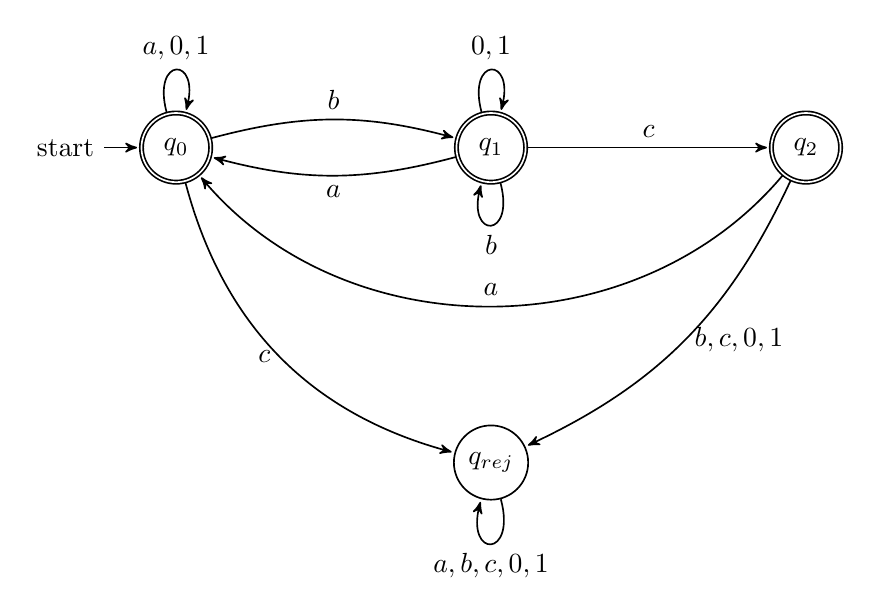
\begin{tikzpicture}[>=stealth', shorten >=1pt, auto, node distance=4cm, semithick]
        \node[state, initial, accepting] (q0) {$q_0$};
        \node[state, accepting] (q1) [right of=q0] {$q_1$};
        \node[state, accepting] (q2) [right of=q1] {$q_2$};
        \node[state] (qrej) [below of=q1, node distance=4cm] {$q_{rej}$};
        
        \path[->]
        % From q0
        (q0) edge[loop above] node {$a,0,1$} (q0)
        (q0) edge[bend left=15] node[above] {$b$} (q1)
        (q0) edge[bend right=30] node[left] {$c$} (qrej)
        
        % From q1 (seen b)
        (q1) edge[loop above] node {$0,1$} (q1)
        (q1) edge node[above] {$c$} (q2)
        (q1) edge[bend left=15] node[below] {$a$} (q0)
        (q1) edge[loop below] node[below] {$b$} (q1)
        
        % From q2 (seen bc)
        (q2) edge[bend left=50] node[above] {$a$} (q0)
        (q2) edge[bend left=20] node[right] {$b,c,0,1$} (qrej)
        
        % Rejection state
        (qrej) edge[loop below] node {$a,b,c,0,1$} (qrej);
    \end{tikzpicture}
\end{center}

\subsection*{2. $\{w \in \Sigma^*_{bool} \mid w = 0^n1^n, n \geq 5\}$}

\textbf{Answer:} This language is not regular.

\textbf{Proof by pumping lemma:}

Assume for contradiction that the language is regular. Let $p$ be the pumping length.

Consider the string $w = 0^{p+5}1^{p+5} \in L$ (since $p+5 \geq 5$).

We have $|w| = 2(p+5) \geq p$, so by the pumping lemma, we can write $w = w_1w_2w_3$ where:
\begin{enumerate}
    \item $|w_1w_2| \leq p$
    \item $|w_2| \geq 1$
    \item $w_1w_2^iw_3 \in L$ for all $i \geq 0$
\end{enumerate}

Since $|w_1w_2| \leq p < p+5$ and $w = 0^{p+5}1^{p+5}$, the substring $w_1w_2$ is entirely 0's. Therefore, $w_2 = 0^k$ for some $k \geq 1$.

Now consider $w_1w_2^0w_3 = w_1w_3 = 0^{p+5-k}1^{p+5}$.

Since $k \geq 1$, we have $p+5-k < p+5$, so the number of 0's is less than the number of 1's.

Therefore, $w_1w_3 \notin L$, which contradicts the pumping lemma.

Therefore, the language is not regular.

\subsection*{3. $\{w \in \Sigma^*_{bool} \mid w = 0^n1^m, n \geq 0, m \geq 1\}$}

\textbf{Answer:} This language is regular.

\begin{center}
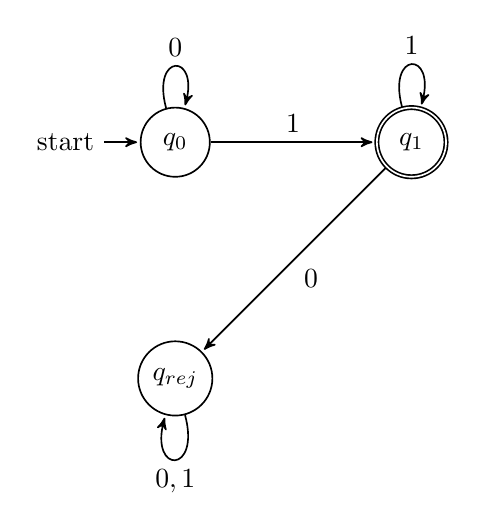
\begin{tikzpicture}[>=stealth', shorten >=1pt, auto, node distance=3cm, semithick]
    \node[state, initial] (q0) {$q_0$};
    \node[state, accepting] (q1) [right of=q0] {$q_1$};
    \node[state] (qrej) [below of=q0] {$q_{rej}$};
    
    \path[->]
    (q0) edge[loop above] node {$0$} (q0)
    (q0) edge node {$1$} (q1)
    (q1) edge[loop above] node {$1$} (q1)
    (q1) edge node {$0$} (qrej)
    (qrej) edge[loop below] node {$0,1$} (qrej);
\end{tikzpicture}
\end{center}

\subsection*{4. $\{w \in \Sigma^*_{bool} \mid w = w_1w_2, w_1 \in 0^*1, w_2 \in 0^*1, \text{ and } |w_1|, |w_2| \geq 1\}$}

\textbf{Answer:} This language is regular.

\begin{center}
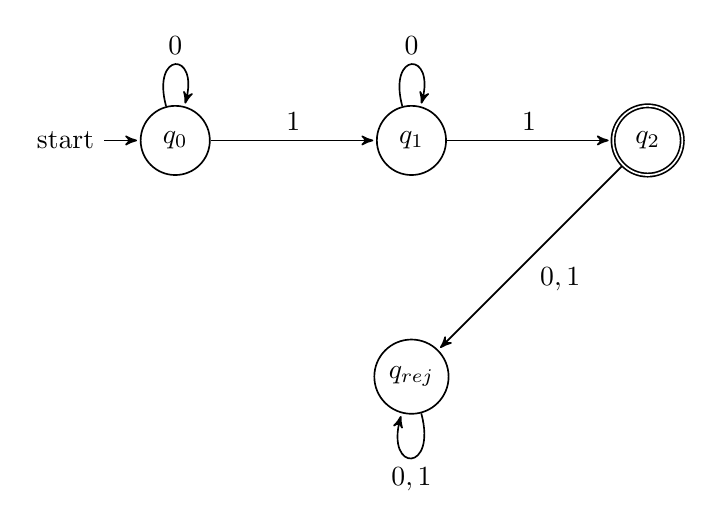
\begin{tikzpicture}[>=stealth', shorten >=1pt, auto, node distance=3cm, semithick]
    \node[state, initial] (q0) {$q_0$};
    \node[state] (q1) [right of=q0] {$q_1$};
    \node[state, accepting] (q2) [right of=q1] {$q_2$};
    \node[state] (qrej) [below of=q1] {$q_{rej}$};
    
    \path[->]
    (q0) edge[loop above] node {$0$} (q0)
    (q0) edge node {$1$} (q1)
    (q1) edge[loop above] node {$0$} (q1)
    (q1) edge node {$1$} (q2)
    (q2) edge node {$0,1$} (qrej)
    (qrej) edge[loop below] node {$0,1$} (qrej);
\end{tikzpicture}
\end{center}

\newpage

\section*{Question 2 (10 points)}

Design a NFA for the following language:
$$L_2 = \{w \in \{a, b, 0, 1\}^* \mid w = w_1a0b1w_2, w_1, w_2 \in \{a, b, 0, 1\}^*\}$$

\textbf{Solution:} The language consists of all strings that contain the substring $a0b1$.

\begin{center}
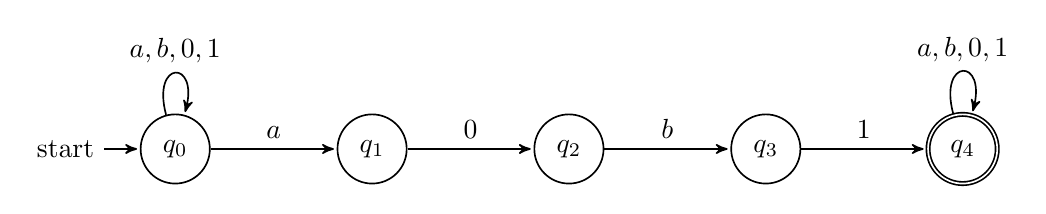
\begin{tikzpicture}[>=stealth', shorten >=1pt, auto, node distance=2.5cm, semithick]
    \node[state, initial] (q0) {$q_0$};
    \node[state] (q1) [right of=q0] {$q_1$};
    \node[state] (q2) [right of=q1] {$q_2$};
    \node[state] (q3) [right of=q2] {$q_3$};
    \node[state, accepting] (q4) [right of=q3] {$q_4$};
    
    \path[->]
    (q0) edge [loop above] node {$a,b,0,1$} (q0)
    (q0) edge node {$a$} (q1)
    (q1) edge node {$0$} (q2)
    (q2) edge node {$b$} (q3)
    (q3) edge node {$1$} (q4)
    (q4) edge [loop above] node {$a,b,0,1$} (q4);
\end{tikzpicture}
\end{center}

\section*{Question 3 (10 points)}

Design a NFA for the following language:
$$L_3 = \{w \in \{a, b, 0, 1\}^* \mid w \text{ ends in the string } ab00\}$$

\textbf{Solution:}

\begin{center}
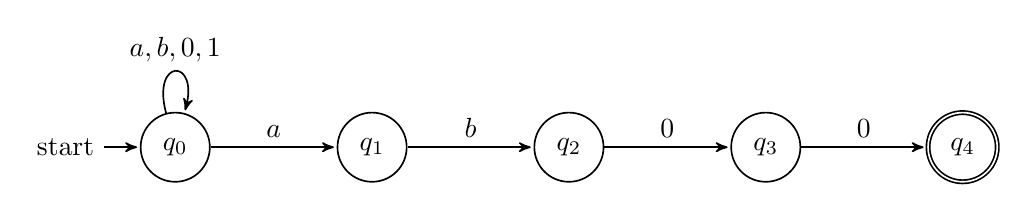
\begin{tikzpicture}[>=stealth', shorten >=1pt, auto, node distance=2.5cm, semithick]
    \node[state, initial] (q0) {$q_0$};
    \node[state] (q1) [right of=q0] {$q_1$};
    \node[state] (q2) [right of=q1] {$q_2$};
    \node[state] (q3) [right of=q2] {$q_3$};
    \node[state, accepting] (q4) [right of=q3] {$q_4$};
    
    \path[->]
    (q0) edge [loop above] node {$a,b,0,1$} (q0)
    (q0) edge node {$a$} (q1)
    (q1) edge node {$b$} (q2)
    (q2) edge node {$0$} (q3)
    (q3) edge node {$0$} (q4);
\end{tikzpicture}
\end{center}

\section*{Question 4 (10 points)}

Design a NFA for the following language:
$$L_4 = \{w \in \{a, b, 0\}^* \mid w \text{ contains the subwords } aba \text{ and } abb\}$$

\textbf{Solution:} The NFA needs to find both substrings $aba$ and $abb$ in the input.

\begin{center}
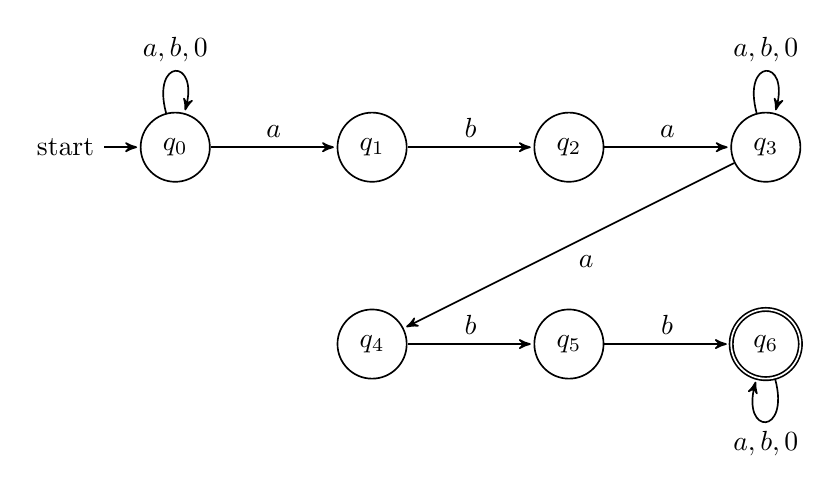
\begin{tikzpicture}[>=stealth', shorten >=1pt, auto, node distance=2.5cm, semithick]
    % Path for finding aba
    \node[state, initial] (q0) {$q_0$};
    \node[state] (q1) [right of=q0] {$q_1$};
    \node[state] (q2) [right of=q1] {$q_2$};
    \node[state] (q3) [right of=q2] {$q_3$};
    
    % Path for finding abb
    \node[state] (q4) [below of=q1] {$q_4$};
    \node[state] (q5) [right of=q4] {$q_5$};
    \node[state, accepting] (q6) [right of=q5] {$q_6$};
    
    \path[->]
    % Stay in q0 until we start matching
    (q0) edge [loop above] node {$a,b,0$} (q0)
    % Path for aba
    (q0) edge node {$a$} (q1)
    (q1) edge node {$b$} (q2)
    (q2) edge node {$a$} (q3)
    (q3) edge [loop above] node {$a,b,0$} (q3)
    % Path for abb from q3
    (q3) edge node {$a$} (q4)
    (q4) edge node {$b$} (q5)
    (q5) edge node {$b$} (q6)
    (q6) edge [loop below] node {$a,b,0$} (q6);
\end{tikzpicture}
\end{center}

\newpage

\section*{Question 5 (20 points)}

Please answer the following sub-questions:

\subsection*{1. Is the set of languages accepted by NFAs equal to, larger, or smaller than the set of languages accepted by DFAs?}

\textbf{Answer:} The set of languages accepted by NFAs is \textbf{equal to} the set of languages accepted by DFAs.

\textbf{Explanation:} NFAs and DFAs are the same in terms of power. For every NFA, there exists a DFA that accepts the same language, and every DFA is an NFA. Therefore, they accept the same class of languages (regular languages).

\subsection*{2. Regular languages are those languages accepted by NFAs, true or false?}

\textbf{Answer:} \textbf{True}.

\textbf{Explanation:} Regular languages are defined as those languages that can be accepted by finite automata (either DFAs or NFAs). Since NFAs and DFAs are the same in terms of power, regular languages are accepted by both.

\subsection*{3. When converting a NFA to a DFA the resulting DFA will always have the same number of states as the NFA, true or false?}

\textbf{Answer:} \textbf{False}.

\textbf{Explanation:} When converting an NFA with $n$ states to a DFA using the subset construction algorithm, the resulting DFA can have up to $2^n$ states
. The DFA may have the same number of states in special cases, but in general it can have a lot more states.

\subsection*{4. The pumping lemma doesn't prove anything about a language being accepted by a NFA. That is, it's only useful for showing a language can't be accepted by a DFA. True or False?}

\textbf{Answer:} \textbf{False}.

\textbf{Explanation:} Since NFAs and DFAs accept regular languages, the pumping lemma applies to both equally. If a language fails the pumping lemma, it cannot be accepted by either a DFA or an NFA. The pumping lemma is a property of regular languages, and is not tied to one or another.

\newpage

\section*{Question 6 (10 points)}

Let $L_6 = \{w \in \Sigma^*_{bool} \mid |w|_0 = 3 \text{ and } (|w|_1 \geq 2 \text{ or } |w|_1 = 0)\}$. Develop a Finite Automaton that recognizes $L_6$.


\begin{center}
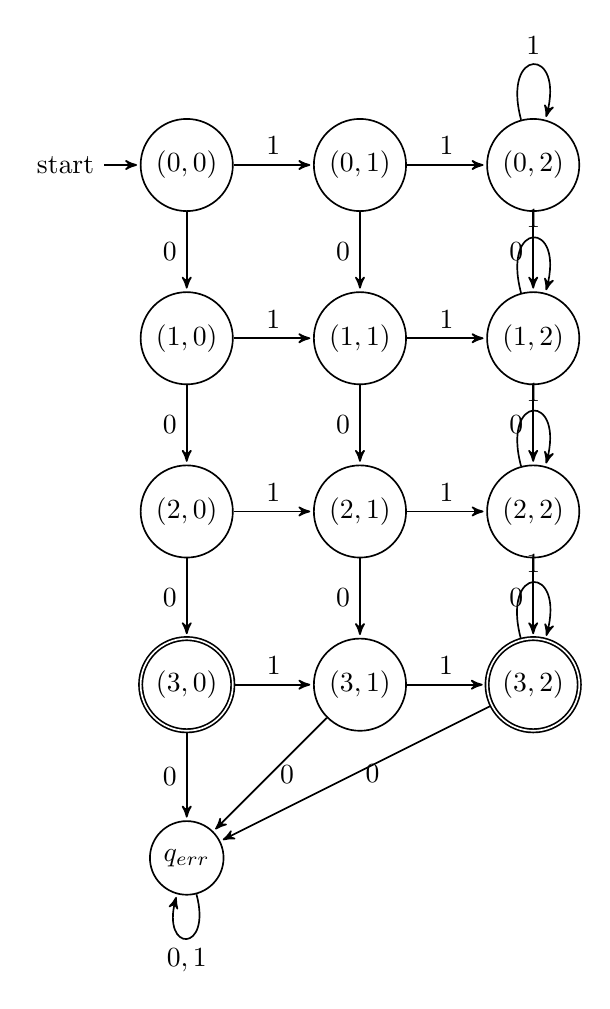
\begin{tikzpicture}[>=stealth', shorten >=1pt, auto, node distance=2.2cm, semithick]
    % Row 0: 0 zeros
    \node[state, initial] (s00) {$(0,0)$};
    \node[state] (s01) [right of=s00] {$(0,1)$};
    \node[state] (s02) [right of=s01] {$(0,2)$};
    
    % Row 1: 1 zero
    \node[state] (s10) [below of=s00] {$(1,0)$};
    \node[state] (s11) [right of=s10] {$(1,1)$};
    \node[state] (s12) [right of=s11] {$(1,2)$};
    
    % Row 2: 2 zeros
    \node[state] (s20) [below of=s10] {$(2,0)$};
    \node[state] (s21) [right of=s20] {$(2,1)$};
    \node[state] (s22) [right of=s21] {$(2,2)$};
    
    % Row 3: 3 zeros (accepting states)
    \node[state, accepting] (s30) [below of=s20] {$(3,0)$};
    \node[state] (s31) [right of=s30] {$(3,1)$};
    \node[state, accepting] (s32) [right of=s31] {$(3,2)$};
    
    % Error state: >3 zeros
    \node[state] (serr) [below of=s30] {$q_{err}$};
    
    % Transitions on 1 (horizontal)
    \path[->]
    (s00) edge node[above] {$1$} (s01)
    (s01) edge node[above] {$1$} (s02)
    (s02) edge[loop above] node {$1$} (s02)
    (s10) edge node[above] {$1$} (s11)
    (s11) edge node[above] {$1$} (s12)
    (s12) edge[loop above] node {$1$} (s12)
    (s20) edge node[above] {$1$} (s21)
    (s21) edge node[above] {$1$} (s22)
    (s22) edge[loop above] node {$1$} (s22)
    (s30) edge node[above] {$1$} (s31)
    (s31) edge node[above] {$1$} (s32)
    (s32) edge[loop above] node {$1$} (s32);
    
    % Transitions on 0 (vertical)
    \path[->]
    (s00) edge node[left] {$0$} (s10)
    (s01) edge node[left] {$0$} (s11)
    (s02) edge node[left] {$0$} (s12)
    (s10) edge node[left] {$0$} (s20)
    (s11) edge node[left] {$0$} (s21)
    (s12) edge node[left] {$0$} (s22)
    (s20) edge node[left] {$0$} (s30)
    (s21) edge node[left] {$0$} (s31)
    (s22) edge node[left] {$0$} (s32)
    (s30) edge node[left] {$0$} (serr)
    (s31) edge node[right] {$0$} (serr)
    (s32) edge node[right] {$0$} (serr)
    (serr) edge[loop below] node {$0,1$} (serr);
\end{tikzpicture}
\end{center}

\section*{Question 7 (10 points)}

Convert the following NFA to a DFA:

\textbf{Solution DFA:}

\begin{center}
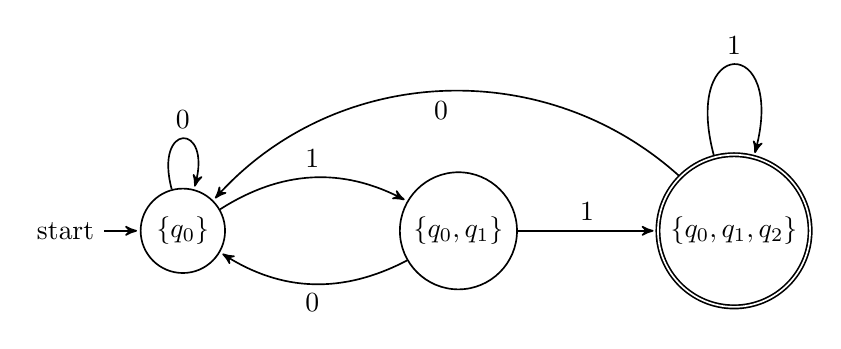
\begin{tikzpicture}[>=stealth', shorten >=1pt, auto, node distance=3.5cm, semithick]
    \node[state, initial] (A) {$\{q_0\}$};
    \node[state] (B) [right of=A] {$\{q_0,q_1\}$};
    \node[state, accepting] (C) [right of=B] {$\{q_0,q_1,q_2\}$};
    
    \path[->]
    (A) edge[loop above] node {$0$} (A)
    (A) edge[bend left] node[above] {$1$} (B)
    (B) edge[bend left] node[below] {$0$} (A)
    (B) edge node[above] {$1$} (C)
    (C) edge[bend right=45] node[below] {$0$} (A)
    (C) edge[loop above] node {$1$} (C);
\end{tikzpicture}
\end{center}

\section*{Question 8 (10 points)}

In-class we developed an algorithm that converts any NFA into a DFA. Why is there no algorithm to convert any DFA into an NFA?

\textbf{Answer:}

There is no need for such an algorithm because \textbf{every DFA is already an NFA}.


A DFA is a special case of an NFA where there are no $\epsilon$ transitions and for each state and each input symbol, there is exactly one transition.
Since the definition of an NFA is more general than a DFA, any DFA could technically be an NFA. 


\end{document}